\documentclass{standalone}
\usepackage{tikz}
\usetikzlibrary{patterns, positioning}
\usepackage[sfdefault]{ClearSans} %% option 'sfdefault' activates Clear Sans as the default text font
\usepackage[T1]{fontenc}

\begin{document}
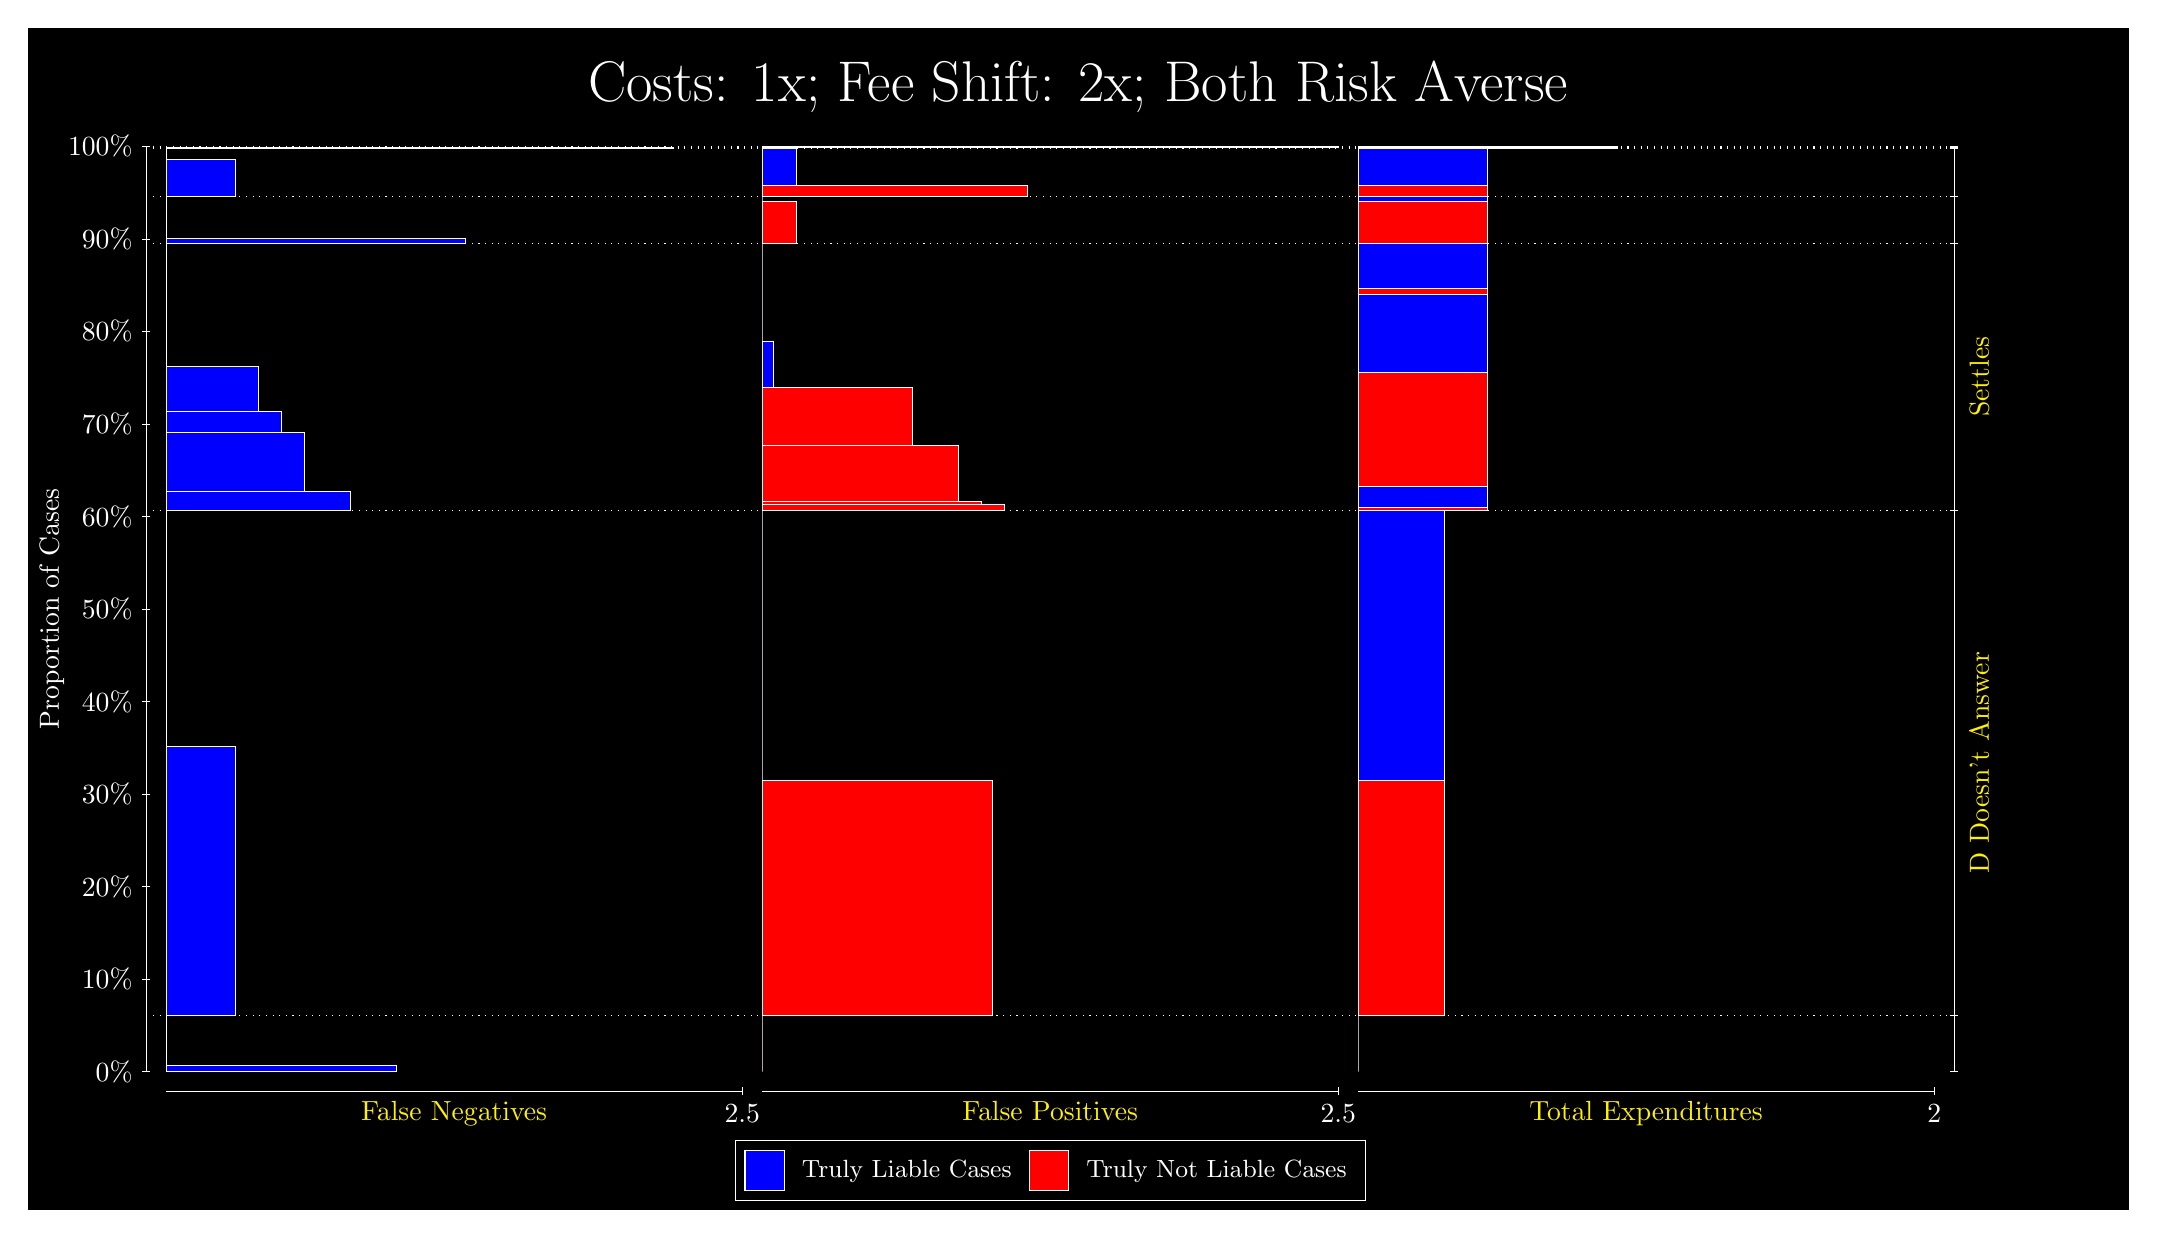
\begin{tikzpicture}
\draw[fill=black] (0,0) rectangle (26.667,15);
\draw[text=white] (0,13.5) rectangle (26.667,15) node[midway] {\huge Costs: 1x; Fee Shift: 2x; Both Risk Averse};
\draw[white, very thin] (1.5,1.75) -- (1.5,13.5);
\node[rotate=90, text=white, anchor=center] at (0.3, 7.625) {Proportion of Cases};
\draw[white, very thin] (1.45,1.75) -- (1.55,1.75);
\node[text=white, anchor=east] at (1.45, 1.75) {0\%};
\draw[white, very thin] (1.45,2.925) -- (1.55,2.925);
\node[text=white, anchor=east] at (1.45, 2.925) {10\%};
\draw[white, very thin] (1.45,4.1) -- (1.55,4.1);
\node[text=white, anchor=east] at (1.45, 4.1) {20\%};
\draw[white, very thin] (1.45,5.275) -- (1.55,5.275);
\node[text=white, anchor=east] at (1.45, 5.275) {30\%};
\draw[white, very thin] (1.45,6.45) -- (1.55,6.45);
\node[text=white, anchor=east] at (1.45, 6.45) {40\%};
\draw[white, very thin] (1.45,7.625) -- (1.55,7.625);
\node[text=white, anchor=east] at (1.45, 7.625) {50\%};
\draw[white, very thin] (1.45,8.8) -- (1.55,8.8);
\node[text=white, anchor=east] at (1.45, 8.8) {60\%};
\draw[white, very thin] (1.45,9.975) -- (1.55,9.975);
\node[text=white, anchor=east] at (1.45, 9.975) {70\%};
\draw[white, very thin] (1.45,11.15) -- (1.55,11.15);
\node[text=white, anchor=east] at (1.45, 11.15) {80\%};
\draw[white, very thin] (1.45,12.325) -- (1.55,12.325);
\node[text=white, anchor=east] at (1.45, 12.325) {90\%};
\draw[white, very thin] (1.45,13.5) -- (1.55,13.5);
\node[text=white, anchor=east] at (1.45, 13.5) {100\%};

\draw[white, very thin] (24.457,1.75) -- (24.457,13.5);
\draw[white, very thin] (24.407,1.75) -- (24.507,1.75);
\node[anchor=west] at (24.407, 1.75) {};
\draw[white, very thin] (24.407,2.4592) -- (24.507,2.4592);
\node[anchor=west] at (24.407, 2.4592) {};
\draw[white, very thin] (24.407,8.8796) -- (24.507,8.8796);
\node[anchor=west] at (24.407, 8.8796) {};
\draw[white, very thin] (24.407,12.269) -- (24.507,12.269);
\node[anchor=west] at (24.407, 12.269) {};
\draw[white, very thin] (24.407,12.868) -- (24.507,12.868);
\node[anchor=west] at (24.407, 12.868) {};
\draw[white, very thin] (24.407,13.479) -- (24.507,13.479);
\node[anchor=west] at (24.407, 13.479) {};
\draw[white, very thin] (24.407,13.492) -- (24.507,13.492);
\node[anchor=west] at (24.407, 13.492) {};
\draw[white, very thin] (24.407,13.5) -- (24.507,13.5);
\node[anchor=west] at (24.407, 13.5) {};

\draw[white, very thin, fill=blue] (1.75,1.75) rectangle (4.6775,1.8246);
\draw[white, very thin, fill=red] (1.75,1.8246) rectangle (1.75,2.4592);
\draw[white, very thin, fill=blue] (1.75,2.4592) rectangle (2.6283,5.8851);
\draw[white, very thin, fill=red] (1.75,5.8851) rectangle (1.75,8.8796);
\draw[white, very thin, fill=blue] (1.75,8.8796) rectangle (4.092,9.1183);
\draw[white, very thin, fill=blue] (1.75,9.1183) rectangle (3.5065,9.8711);
\draw[white, very thin, fill=blue] (1.75,9.8711) rectangle (3.2138,10.131);
\draw[white, very thin, fill=blue] (1.75,10.131) rectangle (2.921,10.706);
\draw[white, very thin, fill=red] (1.75,10.706) rectangle (1.75,12.269);
\draw[white, very thin, fill=blue] (1.75,12.269) rectangle (5.5558,12.338);
\draw[white, very thin, fill=red] (1.75,12.338) rectangle (1.75,12.868);
\draw[white, very thin, fill=blue] (1.75,12.868) rectangle (2.6283,13.338);
\draw[white, very thin, fill=red] (1.75,13.338) rectangle (1.75,13.479);
\draw[white, very thin, fill=blue] (1.75,13.479) rectangle (8.1906,13.483);
\draw[white, very thin, fill=red] (1.75,13.483) rectangle (1.75,13.492);
\draw[white, very thin, fill=red] (1.75,13.492) rectangle (1.75,13.496);
\draw[white, very thin, fill=blue] (1.75,13.496) rectangle (1.75,13.5);
\draw[white, very thin, fill=red] (9.3189,1.75) rectangle (9.3189,2.3846);
\draw[white, very thin, fill=blue] (9.3189,2.3846) rectangle (9.3189,2.4592);
\draw[white, very thin, fill=red] (9.3189,2.4592) rectangle (12.246,5.4537);
\draw[white, very thin, fill=blue] (9.3189,5.4537) rectangle (9.3189,8.8796);
\draw[white, very thin, fill=red] (9.3189,8.8796) rectangle (12.393,8.95);
\draw[white, very thin, fill=red] (9.3189,8.95) rectangle (12.1,8.9901);
\draw[white, very thin, fill=red] (9.3189,8.9901) rectangle (11.807,9.6973);
\draw[white, very thin, fill=red] (9.3189,9.6973) rectangle (11.222,10.443);
\draw[white, very thin, fill=blue] (9.3189,10.443) rectangle (9.4652,11.018);
\draw[white, very thin, fill=blue] (9.3189,11.018) rectangle (9.3189,12.269);
\draw[white, very thin, fill=red] (9.3189,12.269) rectangle (9.758,12.798);
\draw[white, very thin, fill=blue] (9.3189,12.798) rectangle (9.3189,12.868);
\draw[white, very thin, fill=red] (9.3189,12.868) rectangle (12.686,13.008);
\draw[white, very thin, fill=blue] (9.3189,13.008) rectangle (9.758,13.479);
\draw[white, very thin, fill=red] (9.3189,13.479) rectangle (9.3189,13.489);
\draw[white, very thin, fill=blue] (9.3189,13.489) rectangle (9.3189,13.492);
\draw[white, very thin, fill=red] (9.3189,13.492) rectangle (16.638,13.496);
\draw[white, very thin, fill=blue] (9.3189,13.496) rectangle (13.71,13.5);
\draw[white, very thin, fill=red] (16.888,1.75) rectangle (16.888,2.3846);
\draw[white, very thin, fill=blue] (16.888,2.3846) rectangle (16.888,2.4592);
\draw[white, very thin, fill=red] (16.888,2.4592) rectangle (17.986,5.4537);
\draw[white, very thin, fill=blue] (16.888,5.4537) rectangle (17.986,8.8796);
\draw[white, very thin, fill=red] (16.888,8.8796) rectangle (18.534,8.9197);
\draw[white, very thin, fill=blue] (16.888,8.9197) rectangle (18.534,9.1791);
\draw[white, very thin, fill=red] (16.888,9.1791) rectangle (18.534,10.631);
\draw[white, very thin, fill=blue] (16.888,10.631) rectangle (18.534,11.623);
\draw[white, very thin, fill=red] (16.888,11.623) rectangle (18.534,11.693);
\draw[white, very thin, fill=blue] (16.888,11.693) rectangle (18.534,12.269);
\draw[white, very thin, fill=red] (16.888,12.269) rectangle (18.534,12.798);
\draw[white, very thin, fill=blue] (16.888,12.798) rectangle (18.534,12.868);
\draw[white, very thin, fill=red] (16.888,12.868) rectangle (18.534,13.008);
\draw[white, very thin, fill=blue] (16.888,13.008) rectangle (18.534,13.479);
\draw[white, very thin, fill=red] (16.888,13.479) rectangle (20.181,13.489);
\draw[white, very thin, fill=blue] (16.888,13.489) rectangle (20.181,13.492);
\draw[white, very thin, fill=red] (16.888,13.492) rectangle (20.181,13.496);
\draw[white, very thin, fill=blue] (16.888,13.496) rectangle (20.181,13.5);
\draw[white, dotted] (1.5,2.4592) -- (24.457,2.4592);
\draw[white, dotted] (1.5,8.8796) -- (24.457,8.8796);
\draw[white, dotted] (1.5,12.269) -- (24.457,12.269);
\draw[white, dotted] (1.5,12.868) -- (24.457,12.868);
\draw[white, dotted] (1.5,13.479) -- (24.457,13.479);
\draw[white, dotted] (1.5,13.492) -- (24.457,13.492);
\draw[white, very thin] (1.75,1.5) -- (9.0689,1.5);
\node[text=yellow, anchor=north] at (5.4094, 1.5) {False Negatives};
\draw[white, very thin] (9.0689,1.45) -- (9.0689,1.55);
\node[text=white, anchor=north] at (9.0689, 1.45) {2.5};

\draw[white, very thin] (9.3189,1.5) -- (16.638,1.5);
\node[text=yellow, anchor=north] at (12.978, 1.5) {False Positives};
\draw[white, very thin] (16.638,1.45) -- (16.638,1.55);
\node[text=white, anchor=north] at (16.638, 1.45) {2.5};

\draw[white, very thin] (16.888,1.5) -- (24.207,1.5);
\node[text=yellow, anchor=north] at (20.547, 1.5) {Total Expenditures};
\draw[white, very thin] (24.207,1.45) -- (24.207,1.55);
\node[text=white, anchor=north] at (24.207, 1.45) {2};


\node[text=yellow, centered, rotate=90] at (24.777, 5.6694) {D Doesn't Answer};
\node[text=yellow, centered, rotate=90] at (24.777, 10.574) {Settles};





\draw (12.978300999999998,1.5) node[draw=none] (baseCoordinate) {};
\begin{scope}[align=center]
        \matrix[scale=0.5, draw=white, below=0.5cm of baseCoordinate, nodes={draw}, column sep=0.1cm]{
            \node[rectangle, draw, minimum width=0.5cm, minimum height=0.5cm, fill=blue] {}; &
            \node[draw=none, font=\small, text=white] (B) {Truly Liable Cases}; &
            \node[rectangle, draw, minimum width=0.5cm, minimum height=0.5cm, fill=red] {}; &
            \node[draw=none, font=\small, text=white] (B) {Truly Not Liable Cases}; \\
            };
\end{scope}

\end{tikzpicture}
\end{document}